\documentclass{standalone}
\usepackage{tikz}
\usetikzlibrary{patterns, positioning}
\usepackage[sfdefault]{ClearSans} %% option 'sfdefault' activates Clear Sans as the default text font
\usepackage[T1]{fontenc}

\begin{document}
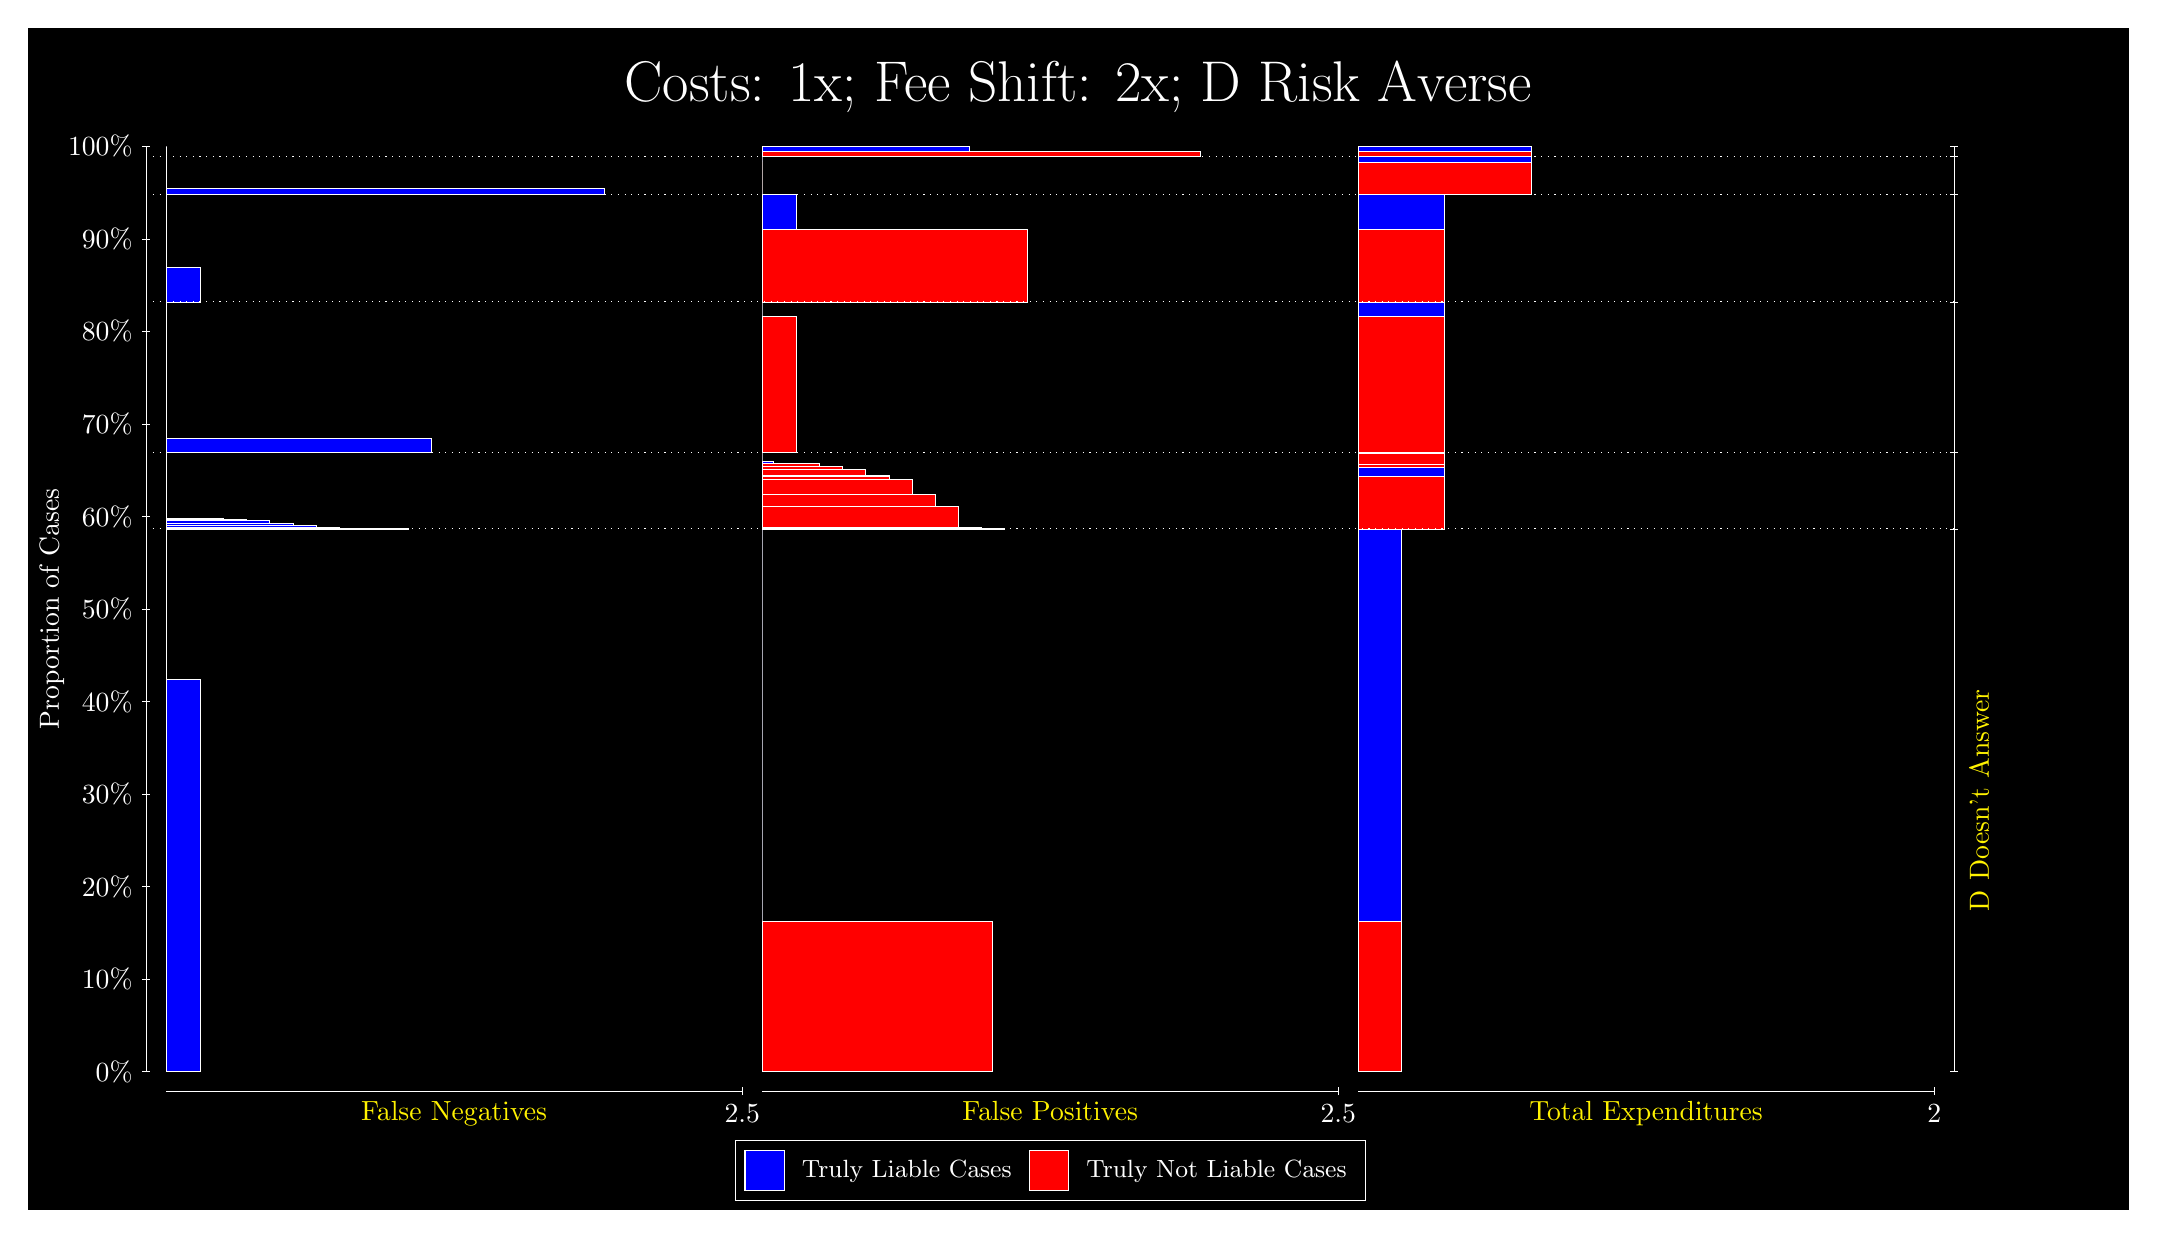
\begin{tikzpicture}
\draw[fill=black] (0,0) rectangle (26.667,15);
\draw[text=white] (0,13.5) rectangle (26.667,15) node[midway] {\huge Costs: 1x; Fee Shift: 2x; D Risk Averse};
\draw[white, very thin] (1.5,1.75) -- (1.5,13.5);
\node[rotate=90, text=white, anchor=center] at (0.3, 7.625) {Proportion of Cases};
\draw[white, very thin] (1.45,1.75) -- (1.55,1.75);
\node[text=white, anchor=east] at (1.45, 1.75) {0\%};
\draw[white, very thin] (1.45,2.925) -- (1.55,2.925);
\node[text=white, anchor=east] at (1.45, 2.925) {10\%};
\draw[white, very thin] (1.45,4.1) -- (1.55,4.1);
\node[text=white, anchor=east] at (1.45, 4.1) {20\%};
\draw[white, very thin] (1.45,5.275) -- (1.55,5.275);
\node[text=white, anchor=east] at (1.45, 5.275) {30\%};
\draw[white, very thin] (1.45,6.45) -- (1.55,6.45);
\node[text=white, anchor=east] at (1.45, 6.45) {40\%};
\draw[white, very thin] (1.45,7.625) -- (1.55,7.625);
\node[text=white, anchor=east] at (1.45, 7.625) {50\%};
\draw[white, very thin] (1.45,8.8) -- (1.55,8.8);
\node[text=white, anchor=east] at (1.45, 8.8) {60\%};
\draw[white, very thin] (1.45,9.975) -- (1.55,9.975);
\node[text=white, anchor=east] at (1.45, 9.975) {70\%};
\draw[white, very thin] (1.45,11.15) -- (1.55,11.15);
\node[text=white, anchor=east] at (1.45, 11.15) {80\%};
\draw[white, very thin] (1.45,12.325) -- (1.55,12.325);
\node[text=white, anchor=east] at (1.45, 12.325) {90\%};
\draw[white, very thin] (1.45,13.5) -- (1.55,13.5);
\node[text=white, anchor=east] at (1.45, 13.5) {100\%};

\draw[white, very thin] (24.457,1.75) -- (24.457,13.5);
\draw[white, very thin] (24.407,1.75) -- (24.507,1.75);
\node[anchor=west] at (24.407, 1.75) {};
\draw[white, very thin] (24.407,8.6415) -- (24.507,8.6415);
\node[anchor=west] at (24.407, 8.6415) {};
\draw[white, very thin] (24.407,9.6136) -- (24.507,9.6136);
\node[anchor=west] at (24.407, 9.6136) {};
\draw[white, very thin] (24.407,11.525) -- (24.507,11.525);
\node[anchor=west] at (24.407, 11.525) {};
\draw[white, very thin] (24.407,12.892) -- (24.507,12.892);
\node[anchor=west] at (24.407, 12.892) {};
\draw[white, very thin] (24.407,13.372) -- (24.507,13.372);
\node[anchor=west] at (24.407, 13.372) {};
\draw[white, very thin] (24.407,13.5) -- (24.507,13.5);
\node[anchor=west] at (24.407, 13.5) {};

\draw[white, very thin, fill=blue] (1.75,1.75) rectangle (2.1891,6.7308);
\draw[white, very thin, fill=red] (1.75,6.7308) rectangle (1.75,8.6415);
\draw[white, very thin, fill=blue] (1.75,8.6415) rectangle (4.8239,8.6443);
\draw[white, very thin, fill=blue] (1.75,8.6443) rectangle (4.5312,8.6475);
\draw[white, very thin, fill=blue] (1.75,8.6475) rectangle (4.2384,8.655);
\draw[white, very thin, fill=blue] (1.75,8.655) rectangle (3.9457,8.6613);
\draw[white, very thin, fill=blue] (1.75,8.6613) rectangle (3.6529,8.6865);
\draw[white, very thin, fill=blue] (1.75,8.6865) rectangle (3.3602,8.7079);
\draw[white, very thin, fill=blue] (1.75,8.7079) rectangle (3.0674,8.7548);
\draw[white, very thin, fill=blue] (1.75,8.7548) rectangle (2.7746,8.7573);
\draw[white, very thin, fill=blue] (1.75,8.7573) rectangle (2.4819,8.778);
\draw[white, very thin, fill=red] (1.75,8.778) rectangle (1.75,9.6136);
\draw[white, very thin, fill=blue] (1.75,9.6136) rectangle (5.1167,9.7975);
\draw[white, very thin, fill=red] (1.75,9.7975) rectangle (1.75,11.525);
\draw[white, very thin, fill=blue] (1.75,11.525) rectangle (2.1891,11.969);
\draw[white, very thin, fill=red] (1.75,11.969) rectangle (1.75,12.892);
\draw[white, very thin, fill=blue] (1.75,12.892) rectangle (7.3123,12.962);
\draw[white, very thin, fill=red] (1.75,12.962) rectangle (1.75,13.372);
\draw[white, very thin, fill=red] (1.75,13.372) rectangle (1.75,13.441);
\draw[white, very thin, fill=blue] (1.75,13.441) rectangle (1.75,13.5);
\draw[white, very thin, fill=red] (9.3189,1.75) rectangle (12.246,3.6607);
\draw[white, very thin, fill=blue] (9.3189,3.6607) rectangle (9.3189,8.6415);
\draw[white, very thin, fill=red] (9.3189,8.6415) rectangle (12.393,8.6549);
\draw[white, very thin, fill=red] (9.3189,8.6549) rectangle (12.1,8.6615);
\draw[white, very thin, fill=red] (9.3189,8.6615) rectangle (11.807,8.9344);
\draw[white, very thin, fill=red] (9.3189,8.9344) rectangle (11.515,9.0869);
\draw[white, very thin, fill=red] (9.3189,9.0869) rectangle (11.222,9.2751);
\draw[white, very thin, fill=red] (9.3189,9.2751) rectangle (10.929,9.3066);
\draw[white, very thin, fill=red] (9.3189,9.3066) rectangle (10.929,9.3269);
\draw[white, very thin, fill=red] (9.3189,9.3269) rectangle (10.636,9.4023);
\draw[white, very thin, fill=red] (9.3189,9.4023) rectangle (10.344,9.4389);
\draw[white, very thin, fill=red] (9.3189,9.4389) rectangle (10.051,9.4771);
\draw[white, very thin, fill=blue] (9.3189,9.4771) rectangle (9.4652,9.4978);
\draw[white, very thin, fill=blue] (9.3189,9.4978) rectangle (9.3189,9.6136);
\draw[white, very thin, fill=red] (9.3189,9.6136) rectangle (9.758,11.341);
\draw[white, very thin, fill=blue] (9.3189,11.341) rectangle (9.3189,11.525);
\draw[white, very thin, fill=red] (9.3189,11.525) rectangle (12.686,12.448);
\draw[white, very thin, fill=blue] (9.3189,12.448) rectangle (9.758,12.892);
\draw[white, very thin, fill=red] (9.3189,12.892) rectangle (9.3189,13.302);
\draw[white, very thin, fill=blue] (9.3189,13.302) rectangle (9.3189,13.372);
\draw[white, very thin, fill=red] (9.3189,13.372) rectangle (14.881,13.441);
\draw[white, very thin, fill=blue] (9.3189,13.441) rectangle (11.954,13.5);
\draw[white, very thin, fill=red] (16.888,1.75) rectangle (17.437,3.6607);
\draw[white, very thin, fill=blue] (16.888,3.6607) rectangle (17.437,8.6415);
\draw[white, very thin, fill=red] (16.888,8.6415) rectangle (17.986,9.3066);
\draw[white, very thin, fill=blue] (16.888,9.3066) rectangle (17.986,9.4271);
\draw[white, very thin, fill=red] (16.888,9.4271) rectangle (17.986,9.4653);
\draw[white, very thin, fill=blue] (16.888,9.4653) rectangle (17.986,9.4681);
\draw[white, very thin, fill=red] (16.888,9.4681) rectangle (17.986,9.6004);
\draw[white, very thin, fill=blue] (16.888,9.6004) rectangle (17.986,9.6136);
\draw[white, very thin, fill=red] (16.888,9.6136) rectangle (17.986,11.341);
\draw[white, very thin, fill=blue] (16.888,11.341) rectangle (17.986,11.525);
\draw[white, very thin, fill=red] (16.888,11.525) rectangle (17.986,12.448);
\draw[white, very thin, fill=blue] (16.888,12.448) rectangle (17.986,12.892);
\draw[white, very thin, fill=red] (16.888,12.892) rectangle (19.083,13.302);
\draw[white, very thin, fill=blue] (16.888,13.302) rectangle (19.083,13.372);
\draw[white, very thin, fill=red] (16.888,13.372) rectangle (19.083,13.441);
\draw[white, very thin, fill=blue] (16.888,13.441) rectangle (19.083,13.5);
\draw[white, dotted] (1.5,8.6415) -- (24.457,8.6415);
\draw[white, dotted] (1.5,9.6136) -- (24.457,9.6136);
\draw[white, dotted] (1.5,11.525) -- (24.457,11.525);
\draw[white, dotted] (1.5,12.892) -- (24.457,12.892);
\draw[white, dotted] (1.5,13.372) -- (24.457,13.372);
\draw[white, very thin] (1.75,1.5) -- (9.0689,1.5);
\node[text=yellow, anchor=north] at (5.4094, 1.5) {False Negatives};
\draw[white, very thin] (9.0689,1.45) -- (9.0689,1.55);
\node[text=white, anchor=north] at (9.0689, 1.45) {2.5};

\draw[white, very thin] (9.3189,1.5) -- (16.638,1.5);
\node[text=yellow, anchor=north] at (12.978, 1.5) {False Positives};
\draw[white, very thin] (16.638,1.45) -- (16.638,1.55);
\node[text=white, anchor=north] at (16.638, 1.45) {2.5};

\draw[white, very thin] (16.888,1.5) -- (24.207,1.5);
\node[text=yellow, anchor=north] at (20.547, 1.5) {Total Expenditures};
\draw[white, very thin] (24.207,1.45) -- (24.207,1.55);
\node[text=white, anchor=north] at (24.207, 1.45) {2};

\node[text=yellow, centered, rotate=90] at (24.777, 5.1958) {D Doesn't Answer};






\draw (12.978300999999998,1.5) node[draw=none] (baseCoordinate) {};
\begin{scope}[align=center]
        \matrix[scale=0.5, draw=white, below=0.5cm of baseCoordinate, nodes={draw}, column sep=0.1cm]{
            \node[rectangle, draw, minimum width=0.5cm, minimum height=0.5cm, fill=blue] {}; &
            \node[draw=none, font=\small, text=white] (B) {Truly Liable Cases}; &
            \node[rectangle, draw, minimum width=0.5cm, minimum height=0.5cm, fill=red] {}; &
            \node[draw=none, font=\small, text=white] (B) {Truly Not Liable Cases}; \\
            };
\end{scope}

\end{tikzpicture}
\end{document}